% Edited conversion of source pp. 40--41.
% The source photographs are represented by compact TikZ schematics.
\ReportHeading
  {Експериментальні дослідження поведінки матеріалу в околі тріщини плоского зразка}
  {А.~П. Дзюба, А.~Г. Пацюк}
  {Дніпровський національний університет імені Олеся Гончара}
  {}

Роботу присвячено розробленню методології дослідження ініціювання, старту та подальшого розвитку тріщин у плоских зразках. Використано поляризаційно-оптичний метод, метод каустик і тіньовий муаровий метод. Зразки виготовляли з оптично активного полікарбонату. Поєднання методів давало змогу отримувати більш інформативну картину поведінки тріщини на різних етапах її розвитку.

Зразок навантажували клином на пресі УП-5 поляризаційно-проєкційної установки ППУ-7 через спеціально підготовлений крайовий надріз, який виконував роль концентратора напружень. Тріщину ініціювали ступінчастим збільшенням навантаження.

\begin{figure}[htbp]
\centering
\begin{tikzpicture}[x=0.72cm,y=0.72cm,line cap=round,line join=round]
  % Panel 1: wedge loading.
  \draw[thick] (0,0) rectangle (2.2,3.0);
  \draw[thick] (1.1,3.0)--(0.72,3.7)--(1.48,3.7)--cycle;
  \draw[thick] (1.1,3.0)--(1.1,1.6);
  \draw[->,thick] (1.1,4.4)--(1.1,3.8);
  \node[font=\scriptsize,align=center] at (1.1,-0.45) {навантаження\\клином};

  % Panel 2: isochromatics.
  \begin{scope}[xshift=3.2cm]
    \draw[thick] (0,0) rectangle (2.2,3.0);
    \draw[thick] (1.1,3.0)--(1.1,1.55);
    \foreach \r in {0.28,0.48,0.70,0.93} {
      \draw (1.1,1.52) ellipse ({1.3*\r} and {0.72*\r});
    }
    \node[font=\scriptsize,align=center] at (1.1,-0.45) {картина\\ізохром};
  \end{scope}

  % Panel 3: prefracture zone.
  \begin{scope}[xshift=6.4cm]
    \draw[thick] (0,0) rectangle (2.2,3.0);
    \draw[thick] (1.1,3.0)--(1.1,1.7);
    \draw[very thick] (1.1,1.7)--(1.1,0.9);
    \fill (1.1,1.45) ellipse (0.18 and 0.55);
    \node[font=\scriptsize,align=center] at (1.1,-0.45) {зона\\передруйнування};
  \end{scope}

  % Panel 4: crack-tip field.
  \begin{scope}[xshift=9.6cm]
    \draw[thick] (0,0) rectangle (2.2,3.0);
    \draw[thick] (1.1,3.0)--(1.1,1.45);
    \foreach \r in {0.25,0.45,0.67,0.90} {
      \draw (1.1,1.42) ellipse ({1.15*\r} and {0.78*\r});
    }
    \node[font=\scriptsize,align=center] at (1.1,-0.45) {поле біля\\вершини};
  \end{scope}
\end{tikzpicture}
\caption{Схематичне відтворення етапів експерименту: клинове навантаження, картина ізохром, зона передруйнування та поле напружень біля вершини тріщини.}
\end{figure}

Перед стартом тріщини формувалася зона передруйнування. Фіксація картин ізохром і каустик давала змогу обчислювати коефіцієнт інтенсивності напружень біля концентратора та аналізувати характер подальшого поширення тріщини.

Щоб зберегти можливість зупинки тріщини й стабілізації її руху, деформації зразка у поперечному напрямку обмежували на віддаленому від тріщини кінці. Через можливе розгалуження тріщини така стабілізація не завжди була успішною.

\begin{figure}[htbp]
\centering
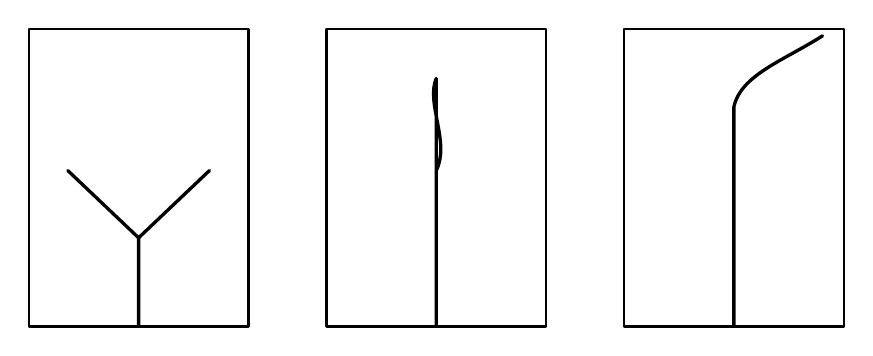
\begin{tikzpicture}[x=0.9cm,y=0.9cm,line cap=round,line join=round]
  \foreach \x in {0,4.2,8.4} {\draw[thick] (\x,0) rectangle ++(3.1,4.2);}
  \draw[very thick] (1.55,0)--(1.55,1.25)--(0.55,2.2);
  \draw[very thick] (1.55,1.25)--(2.55,2.2);
  \draw[very thick] (5.75,0)--(5.75,3.5) .. controls (5.60,3.15) and (5.95,2.6) .. (5.75,2.2);
  \draw[very thick] (9.95,0)--(9.95,3.1) .. controls (10.05,3.55) and (10.65,3.75) .. (11.2,4.1);
\end{tikzpicture}
\caption{Характерні форми поширення тріщини: розгалуження, майже прямолінійний та викривлений шляхи.}
\end{figure}

Отримані результати розширюють експериментальні дані про руйнування тіл із концентраторами напружень і можуть бути використані для верифікації моделей ініціювання та розвитку тріщин.

\textit{Дослідження виконано за підтримки Національного фонду досліджень України, проєкт №~2025.07/0117.}
